
\documentclass[journal,transmag]{IEEEtran}
\hyphenation{op-tical net-works semi-conduc-tor}

\usepackage{enumitem}

% *** GRAPHICS RELATED PACKAGES ***
%
\ifCLASSINFOpdf
   \usepackage[pdftex]{graphicx}
  % declare the path(s) where your graphic files are
  % \graphicspath{{../pdf/}{../jpeg/}}
  % and their extensions so you won't have to specify these with
  % every instance of \includegraphics
  % \DeclareGraphicsExtensions{.pdf,.jpeg,.png}
\else
  % or other class option (dvipsone, dvipdf, if not using dvips). graphicx
  % will default to the driver specified in the system graphics.cfg if no
  % driver is specified.
  % \usepackage[dvips]{graphicx}
  % declare the path(s) where your graphic files are
  % \graphicspath{{../eps/}}
  % and their extensions so you won't have to specify these with
  % every instance of \includegraphics
  % \DeclareGraphicsExtensions{.eps}
\fi
% graphicx was written by David Carlisle and Sebastian Rahtz. It is
% required if you want graphics, photos, etc. graphicx.sty is already
% installed on most LaTeX systems. The latest version and documentation
% can be obtained at: 
% http://www.ctan.org/pkg/graphicx
% Another good source of documentation is "Using Imported Graphics in
% LaTeX2e" by Keith Reckdahl which can be found at:
% http://www.ctan.org/pkg/epslatex
%
% latex, and pdflatex in dvi mode, support graphics in encapsulated
% postscript (.eps) format. pdflatex in pdf mode supports graphics
% in .pdf, .jpeg, .png and .mps (metapost) formats. Users should ensure
% that all non-photo figures use a vector format (.eps, .pdf, .mps) and
% not a bitmapped formats (.jpeg, .png). The IEEE frowns on bitmapped formats
% which can result in "jaggedy"/blurry rendering of lines and letters as
% well as large increases in file sizes.
%
% You can find documentation about the pdfTeX application at:
% http://www.tug.org/applications/pdftex





\begin{document}

\title{\textsc{Caracterización molecular y anotación funcional de una proteína hipotética (GenBank: CAI46211.1) del Homo Sapiens. }}

\author{
\IEEEauthorblockN{Tensile Strength of Materials  }
\IEEEauthorblockA{Pontificia Universidad Javeriana, Bogotá, Colombia}
\IEEEauthorblockA{ Laura Echeverry, Paula Ugueto, William Gómez}

}
% The paper headers
\markboth{BIOINFORMÁTICA. Noviembre 18~2022}%
{Shell \MakeLowercase{\textit{et al.}}: Bare Demo of IEEEtran.cls for IEEE Transactions on Magnetics Journals}
\IEEEtitleabstractindextext{%

	\begin{abstract}

	\end{abstract}
	\begin{IEEEkeywords}
	Proteína hipotética, Análisis bioinformático, Tejido cerebral, C-quinasa, Homo Sapiens.
	 	\end{IEEEkeywords}}


\maketitle
\IEEEdisplaynontitleabstractindextext
\IEEEpeerreviewmaketitle


\section{Introducción}

Esta proteína hipotética fue secuenciada por el Centro de Investigación Alemán de Cáncer junto con la Universidad Ludwig Maximilians en el marco del Proyecto del Genoma Alemán [1]. El principal autor de esta secuenciación es el Profesor Dr. Stefan Wiemann, que ha enfocado sus trabajos en el cáncer de seno. El cáncer, así como muchas otras enfermedades humanas nace de aberraciones genéticas que pueden ser heredadas o pueden ocurrir espontáneamente en células somáticas. Estos defectos causan actividades anormales en los productos de genes y provocan funcionamientos erróneos en interacciones moleculares y celulares, terminando en tumores y progreso del cáncer. El objetivo central de esta unidad de investigación es entender la complejidad de los mecanismos moleculares en la regulación de redes de señalamiento y cómo esto impacta en el desarrollo del cáncer, metástasis y la resistencia a las drogas. 
Para esto se hacen proyectos a gran escala, usando tecnologías genómicas y proteómicas para analizar diferentes genes y proteínas candidatos a influenciar en el tema. Por medio de estos análisis se construye conocimiento que se explota posteriormente para la identificación de nuevos marcadores para diagnóstico y pronóstico, así como para desarrollar estrategias de intervención terapéutica. Es así como el estudio de estas proteínas hipotéticas da luces sobre aquellas que están involucradas en los procesos de metástasis y cáncer de mama, estudiando sus actividades intrínsecas y sus redes con otras proteínas o genes. Los estudios han demostrado que las redes proteicas asociadas a tumores cancerígenos son complejas y que involucran diferentes tipos de células, incluyendo aquellas ubicadas en el microambiente del tumor y aquellas dentro de. Se puede, por lo tanto, estudiar sobre el impacto que tienen perturbaciones individuales a diferentes niveles (ADN, ARN, proteínas, metabolitos, fenotipos) en una gran variedad de vías celulares. Con esto se busca tener un mejor entendimiento de la conectividad entre sistemas de interacción en múltiples capas. Actualmente, de la proteína hipotética CAI46211 se sabe que tiene una longitud de 934 aminoácidos que se encuentra en el ser humano (Homo Sapiens). 
El tejido en el que fue hallada es el cerebral y en etapa de desarrollo fetal. Está altamente relacionada, como veremos a lo largo de este artículo, con una proteína quinasa de unión tipo C. Por lo tanto, hace parte de una familia de proteínas quinasas enzimas (PKC) involucradas en controlar la función de otras proteínas por medio de la fosforilación de los grupos hidroxilos en los residuos de aminoácidos serina y treonina en estas proteínas. Por lo tanto, las enzimas PKC juegan un papel importante en numerosas cascadas de señales de transducción. Con el fin de caracterizar una proteína hipotética haciendo uso de herramientas bioinformáticas se buscó en la base de datos de proteínas de NCBI una proteína hipotética que fuera de nuestro interés para hacer un análisis de caracterización molecular y la anotaciones funcionales de esta proteína, con el fin de identificar su función, ubicación, familia, estructura, dominios, motivos principales y sus 
\section{Metodología}
 \textbf{ Sequence retrival and similarity identification}
 La secuencia de la proteína hipotética fue tomada de la base de datos de NCBI. Se descargó en formato FASTA para poder buscarla en diferentes plataformas que nos acerquen a su caracterización. El primer paso para inferir la función de esta proteína fue buscar similitudes con las herramientas del NCBI, se corrió un BLAST para identificar similitudes.

\textbf{ Multiple sequence alignment and phylogeny analysis}
Se implementó MUSCLE, herramienta del EBI para un análisis comparativo y filogenético entre nuestra proteína hipotética y cinco proteínas homólogas. Adicionalmente con Phylogeny.fr se complementó el alineamiento múltiple.

\textbf{ Physiochemical properties analysis}

Se determinaron las propiedades físico-químicas de la proteína por medio de la plataforma ProtParam, una herramienta que suministra ExPASy. Estas incluyen el peso molecular, el pI teórico, los principales aminoácidos que la componen, su composición atómica, la media vida estimada, su índice de inestabilidad y su índice alifático, el número total de residuos cargados negativa y positivamente y las predicciones de GRAVY (grand average hydropathicity).
\textbf{ Subcellular localization analysis}
Se utilizó DeepLoc para predecir su ubicación, esta parece ser el núcleo. Los resultados se validaron con WoLFPSORT, que arrojó como segunda opción de ubicación citosol-núcleo.

\textbf{ Conserved domain, motif, fold, coil, family, and superfamily identification}
Se corrió la secuencia de la proteína para encontrar en el banco del NCBI algún dominio conservado que pueda indicar las funciones principales de la proteína, así como la familia y superfamilia a la que puede pertenecer. Adicionalmente, se buscó en MOTIF de GenomeNet los motivos identificables en la proteína y utilizando InterPro se identificaron sus términos de Gene Onthogoly, confirmaron presencia de dominos conservados y familias homólogas.

\textbf{ Secondary structure prediction}
La plataforma de PSIPRED nos permitió visualizar la estructura que conforma cada uno de los aminoácidos de la proteína. Del mismo modo, SOPMA arroja información sobre las proporciones de estructuras que se tienen en base a la cantidad de aminoácidos que las conforman.

\textbf{ Three-dimensional structure prediction}
Al haber hallado en las herramientas previas homologías entre esta proteína hipotética y otras, se utilizó el programa Swiss Model para predecir su estructura tridimensional.

ESCRIBIR LO QUE SE HIZO EN ALPHAFOLD

\textbf{ Modal queality assessment}

\textbf{ Active site detection}


\section{Resultados y Discusión}
El flujograma del estudio se muestra en la Figura 1
	\begin{figure}[!h]
		\center
		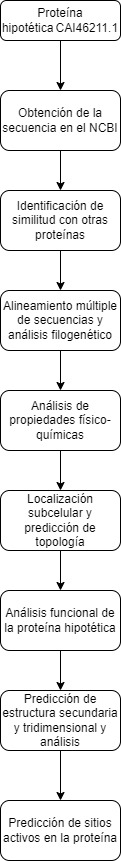
\includegraphics[width=2cm]{imagenes/flujograma.png}
		\caption{Flujograma del trabajo}
		\label{1}
	\end{figure}

\subsection{\textbf{ Sequence and similarity information}}

\begin{figure}[!h]
	\center
	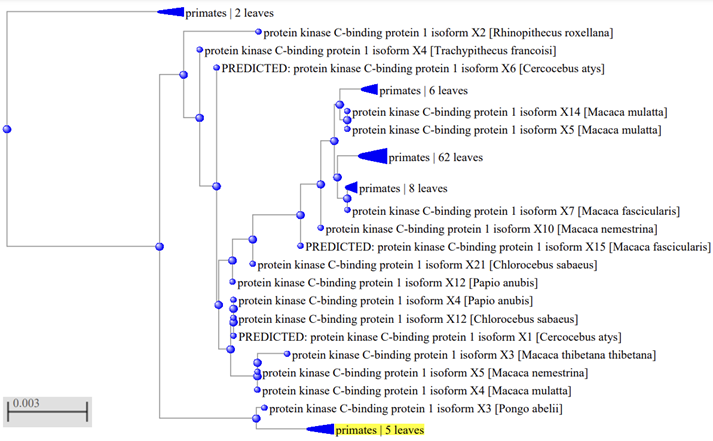
\includegraphics[width=8.5cm]{imagenes/similitudes.png}
	\caption{Árbol con resultados de proteínas similares a la proteína hipotética en cuestión arrojados por Blastp}
	\label{2}
\end{figure}

TABLA 1

\begin{table}[htb]
	\begin{tabular}{|l|l|l|l|l|l|}
	\hline
	Description& Organism & \begin{tabular}[c]{@{}l@{}}Query \\cover\end{tabular}
	& \begin{tabular}[c]{@{}l@{}}E \\value\end{tabular} & \begin{tabular}[c]{@{}l@{}}\% \\identity \end{tabular}
	&  \begin{tabular}[c]{@{}l@{}}Access \\(NCBI)\end{tabular} \\ \hline
	\begin{tabular}[c]{@{}l@{}}protein \\kinase\\C-binding \\protein 1\\isoform \\$CRA_e $\end{tabular}    & \begin{tabular}[c]{@{}l@{}}Homo \\sapiens\end{tabular}&97\%  &0.0   &99.56\%   &\begin{tabular}[c]{@{}l@{}}EAW\\75707.1   \end{tabular}\\ \hline
	\begin{tabular}[c]{@{}l@{}}protein \\kinase\\C-binding \\protein 1\\isoform \\$CRA_k$\end{tabular}   &\begin{tabular}[c]{@{}l@{}}Homo \\sapiens\end{tabular} &97\%   &0.0   &99.56\%   &\begin{tabular}[c]{@{}l@{}}EAW\\75714.1  \end{tabular}\\ \hline
	\begin{tabular}[c]{@{}l@{}}protein \\kinase\\C-binding \\protein 1\\isoform X7\end{tabular}   &\begin{tabular}[c]{@{}l@{}}Pan \\troglodytes \end{tabular}&92\%   &0.0   &96.18\%   &\begin{tabular}[c]{@{}l@{}}XP\_016\\793551.2   \end{tabular}\\ \hline
	\begin{tabular}[c]{@{}l@{}}protein \\kinase\\C-binding \\protein 1\\isoform X3\end{tabular}   &\begin{tabular}[c]{@{}l@{}}Pongo \\abelii \end{tabular}&92\%   &0.0   &95.96\%  &\begin{tabular}[c]{@{}l@{}}XP\_024\\094347.1   \end{tabular}\\ \hline
	\begin{tabular}[c]{@{}l@{}}protein \\kinase\\C-binding \\protein 1\\isoform X3\end{tabular}   & \begin{tabular}[c]{@{}l@{}}Macaca \\thibetana \end{tabular}&92\%   &0.0   &95.17\%   &\begin{tabular}[c]{@{}l@{}}XP\_050\\601089.1  \end{tabular}\\ \hline
	\end{tabular}
\end{table}

\subsection{\textbf{ Multiple sequence alignment and Phylogenetic analysis}}

TABLA 2

\begin{table}[htb]
	\begin{tabular}{|lllllll|}
	\hline
	\multicolumn{7}{|l|}{\begin{tabular}[c]{@{}l@{}}Identity matrix of the hypothetical protein\\ $( tr| Q5JV90|Q5JV90\_HUMAN)$and its 5  most homologous proteins  \end{tabular}}        \\ \hline
	\multicolumn{1}{|l|}{\begin{tabular}[c]{@{}l@{}} XP\_024\\094347.1  \end{tabular}} &100.00  &99.03  &93.42  &91.64   &93.36   &93.79  \\ \cline{1-1}
	\multicolumn{1}{|l|}{\begin{tabular}[c]{@{}l@{}} XP\_050\\601089.1	\end{tabular}} &99.03  &100.00   &92.69   & 91.00  &92.61  &93.04   \\ \cline{1-1}
	\multicolumn{1}{|l|}{\begin{tabular}[c]{@{}l@{}} XP\_016\\793551.2 \end{tabular}}&93.42  &92.69   &100.00   &91.85   &93.58  &94.00   \\ \cline{1-1}
	\multicolumn{1}{|l|}{\begin{tabular}[c]{@{}l@{}} EAW\\75714.1 \end{tabular}}&91.64   &91.00   &91.85   &100.00   &97.53   &97.86   \\ \cline{1-1}
	\multicolumn{1}{|l|}{\begin{tabular}[c]{@{}l@{}} tr|Q5JV90\\|Q5JV90\\\_HUMAN \end{tabular}}&93.36   &92.61  &93.58  &97.53   &100.00   &99.57   \\ \cline{1-1}
	\multicolumn{1}{|l|}{\begin{tabular}[c]{@{}l@{}} EAW\\75707.1 \end{tabular}} &93.79  &93.04   &94.00   &97.86   &99.57   &100.00   \\ \hline
	\end{tabular}
	\end{table}


\begin{figure}[!h]
	\center
	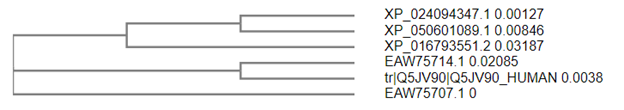
\includegraphics[width=8.5cm]{imagenes/arbol2.png}
	\caption{Figura 3. }
	\label{3}
\end{figure}

\begin{figure}[!h]
	\center
	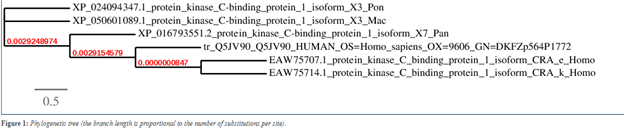
\includegraphics[width=8.5cm]{imagenes/arbol3.png}
	\caption{Figura 4}
	\label{4}
\end{figure}

\subsection{\textbf{ Physicochemical features}}

TABLA 3

\begin{table}[htb]
	\begin{tabular}{|l|l|l|}
	\hline
	 Amino acid& Amount  &Percentage  \\ \hline
	 Ser (S) & 101  & 10.8\%  \\ \hline
	 Lys (K) & 90  & 9.6\%  \\ \hline
	 Pro (P) & 77  & 8.2\%  \\ \hline
	 Glu (E) & 66  & 7.1\%  \\ \hline
	 Thr (T) & 61  & 6.5\%  \\ \hline
	\end{tabular}
	\end{table}


\subsection{\textbf{ Functional annotation of the hypothetical protein}}

\subsection{\textbf{ Subcellular localization nature}}

\begin{figure}[!h]
	\center
	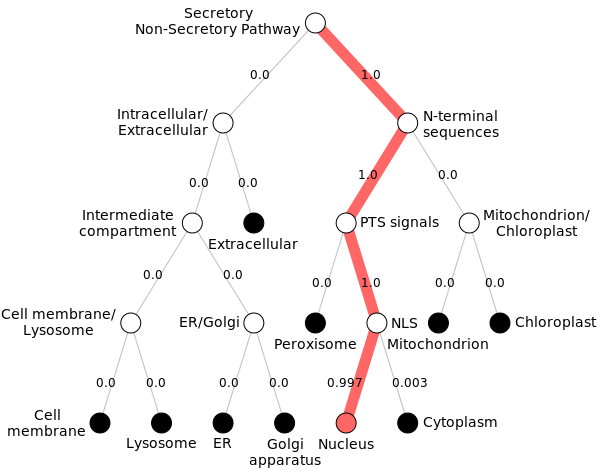
\includegraphics[width=8.5cm]{imagenes/localizacion.png}
	\caption{Ubicación celular de la proteína hipotética}
	\label{5}
\end{figure}

\begin{figure}[!h]
	\center
	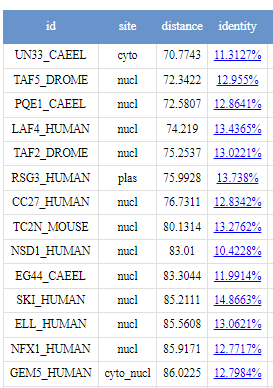
\includegraphics[width=7cm]{imagenes/loca.png}
	\caption{Localizacion celular de WoLFPSORT}
	\label{6}
\end{figure}

\begin{figure}[!h]
	\center
	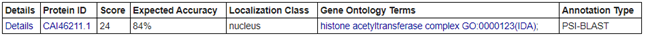
\includegraphics[width=8.5cm]{imagenes/loca2.png}
	\caption{Ubicacion celular de LocTree3}
	\label{7}
\end{figure}

\subsection{\textbf{ Conserved domains, motifs, family and superfamily identification}}

\begin{figure}[!h]
	\center
	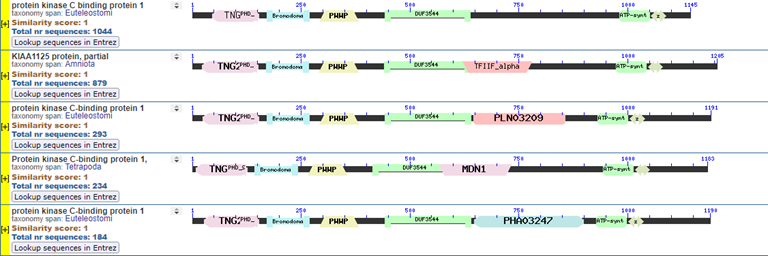
\includegraphics[width=8.5cm]{imagenes/dominios.png}
	\caption{Dominios conservados}
	\label{8}
\end{figure}

\begin{figure}[!h]
	\center
	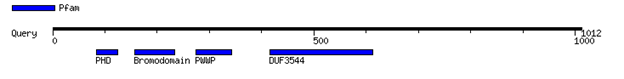
\includegraphics[width=8.5cm]{imagenes/motivos.png}
	\caption{Motivos con InterPro y Pfam}
	\label{9}
\end{figure}



\subsection{\textbf{ Secondary structure analysis}}


\begin{figure}[!h]
	\center
	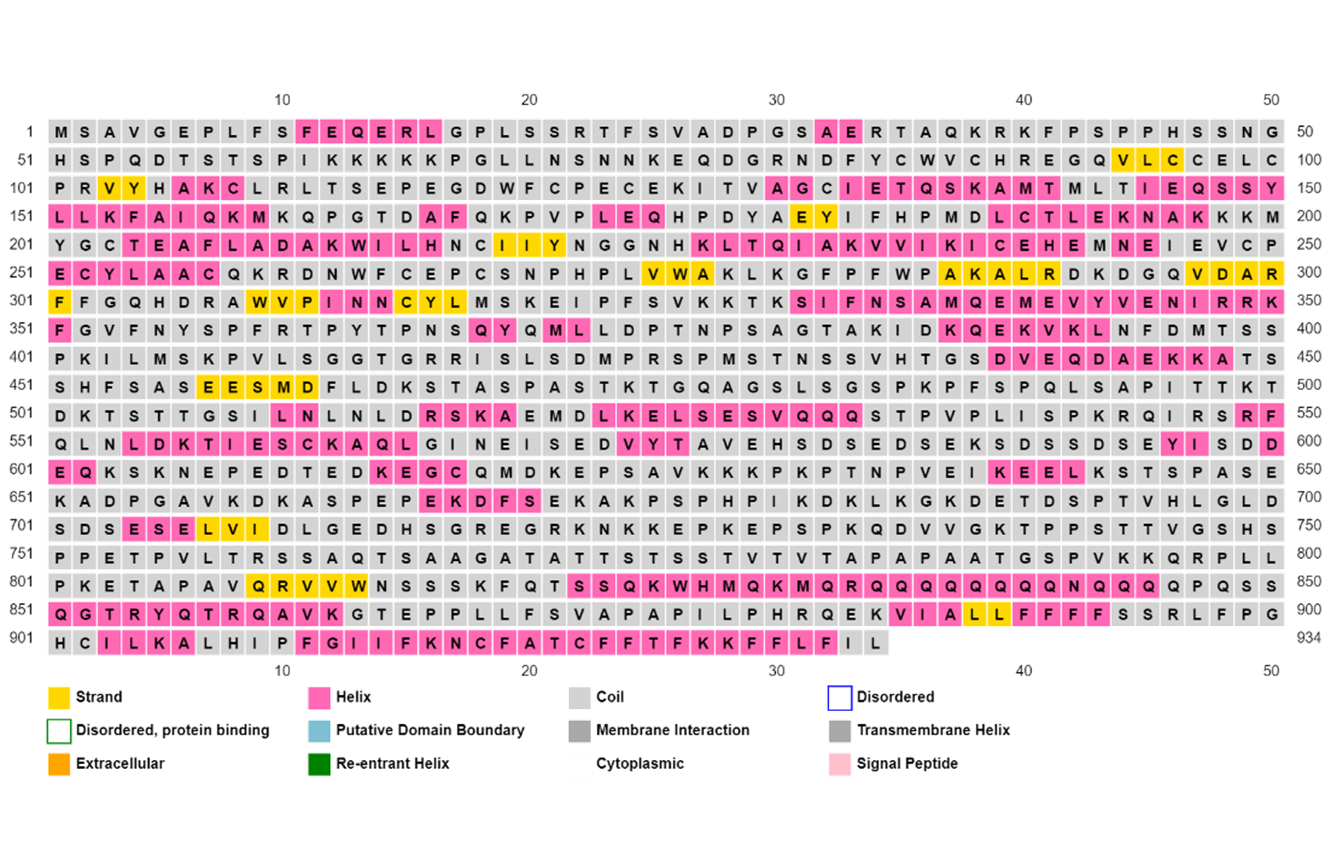
\includegraphics[width=8.5cm]{imagenes/secundaria.png}
	\caption{Configuración de los diferentes aminoácidos que conforman la proteína}
	\label{10}
\end{figure}


TABLA 4
\begin{table}[]
	\begin{tabular}{|l|l|l|}
	\hline
	Alpha Helix & 222 & 23.66\%  \\ \hline
	Extended strand & 129 & 13.81\%  \\ \hline
	Random coil& 555 & 59.42\%  \\ \hline
	Beta turn & 29 & 3.1\%  \\ \hline
	\end{tabular}
	\end{table}

\subsection{\textbf{ Three-dimensional structure analysis}}


\begin{figure}[!h]
	\center
	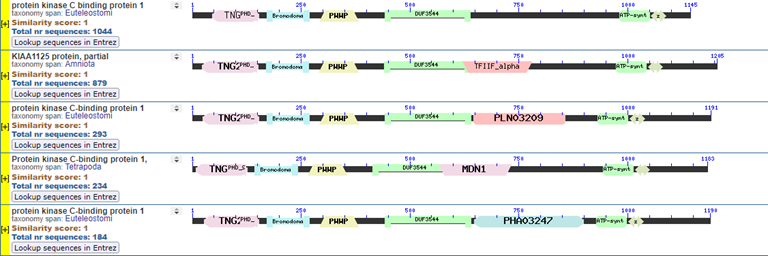
\includegraphics[width=8.5cm]{imagenes/dominios.png}
	\caption{Dominios conservados}
	\label{11}
\end{figure}

\begin{figure}[!h]
	\center
	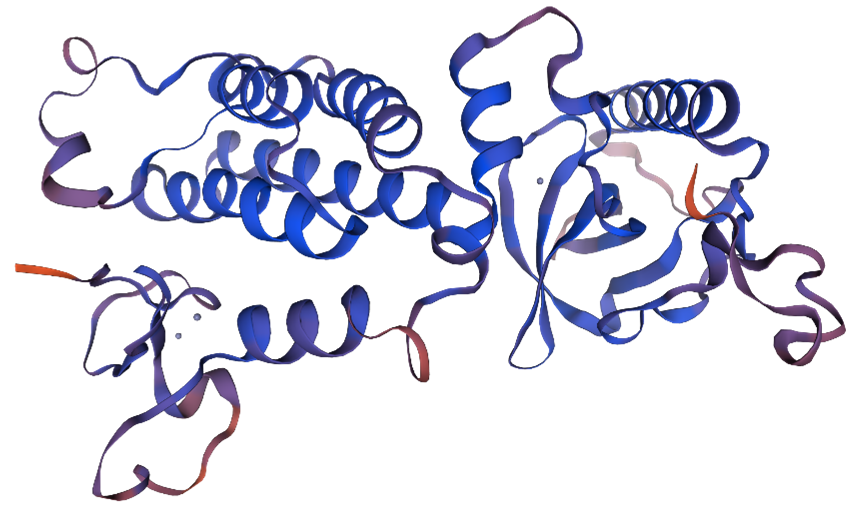
\includegraphics[width=8.5cm]{imagenes/swiss.png}
	\caption{Estructura tridimensional predicha en base a homologías}
	\label{12}
\end{figure}
En esta homología se encuentran las similitudes en cuanto a las hélices Alpha. Sin embargo, se observa que los extremos y algunas zonas no plegadas en forma de hélice difieren en cuanto al modelo elegido. Por lo mismo, el programa arroja otras dos homologías: Transcription intermediary factor 1-alpha (código de acceso 3o35.1.A) y bromodomain PHD finger transcription (código de acceso 2f6j.1.A). Con una identidad del 30.72% y 25.47% respectivamente.  

Sin embargo, se observa en la Figura que una gran parte de la proteína no está modelada, puesto que no se encontraron homólogos que correspondieran a estas zonas. La línea verde es la secuencia de aminoácidos de la proteína hipotética, y toda la zona que no tiene azul por debajo es la que no fue modelada.  

\begin{figure}[!h]
	\center
	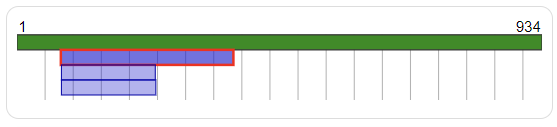
\includegraphics[width=8.5cm]{imagenes/alpha1.png}
	\caption{Coverage of the three-dimensional structure}
	\label{13}
\end{figure}

El resultado que arroja AlphaFold para la estructura tridimensional de la proteína tienen niveles de certeza que corresponden a los resultados de Swiss Model.  

\begin{figure}[!h]
	\center
	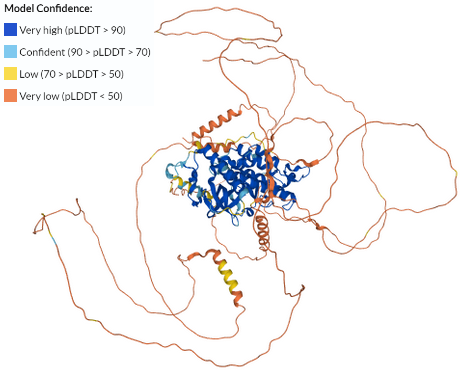
\includegraphics[width=8.5cm]{imagenes/alpha2.png}
	\caption{Confidence of the three-dimensional AlphaFold2 structure}
	\label{14}
\end{figure}
Como se observa en la Figura 14, las zonas de confianza alta son las mismas que aparecen en el modelo anterior, mientras que las de confianza muy baja son las que Swiss Model no modeló por falta de homologías.  

Para corroborar la estructura 3D de la proteína hipotéitca tambien se utilizó phyre2, 

El resultado de esta herramienta es el que se muestra en la imagen a continuación, y se reporta 100\% confidencia en una Cobertura del 33\% de la proteína. Además, se obtiene el tamaño en Armstrong de las dimensiones de la proteína.

\begin{figure}[!h]
	\center
	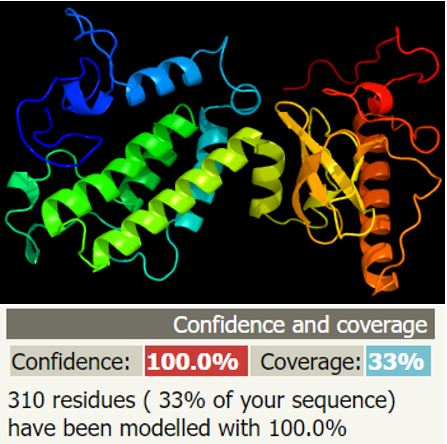
\includegraphics[width=6cm]{imagenes/phyre.JPG}
	\caption{Three-dimensional Phyre2 structure}
	\label{15}
\end{figure}

En PROCHECK y Verify3D se corroboraron los resultados de los modelos obtenidos en las herramientas previamente mencionadas, sin embargo, el resultado no fue positivo. Como se observa en la Figura, apenas 31.48\% de los residuos tuvieron un score 3D-1D superior o igual a 0.2. Como este porcentaje es inferior al 80\%, no se considera que sea un buen modelo.  

\begin{figure}[!h]
	\center
	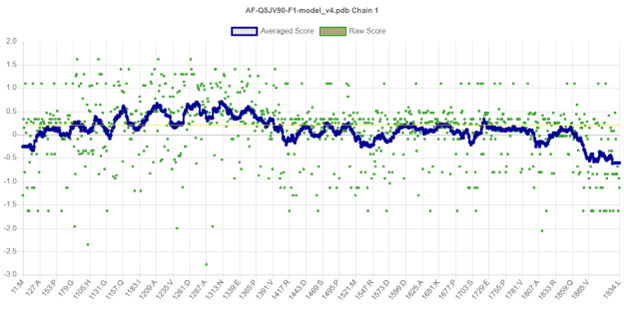
\includegraphics[width=8.5cm]{imagenes/procheck.png}
	\caption{Three-dimensional Phyre2 structure}
	\label{16}
\end{figure}

Por otro lado, PROCHECK arrojó los siguientes resultados: el valor del Ramachandran plot es del 64\%, por lo tanto, no alcanza   el porcentaje de un modelo válido. Como se observa en la Figura , 17.6% de los residuos está en zonas permitidas, pero no muy favorables y el 13.9\% está en zonas no permitidas, que son todos los residuos marcados con su nombre en la Figura.  


\begin{figure}[!h]
	\center
	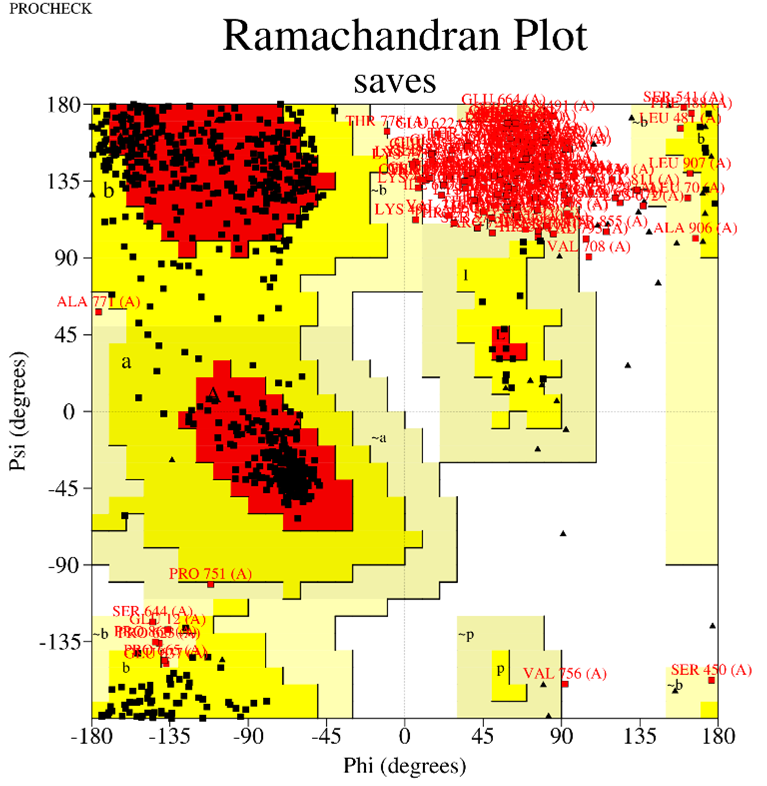
\includegraphics[width=6cm]{imagenes/ramachandran.png}
	\caption{Three-dimensional Phyre2 structure}
	\label{17}
\end{figure}

Estos resultados desfavorables de los modelos tridimensionales de la proteína se deben a que las homologías existentes solo cubren un porcentaje de la proteína hipotética. El resto de la misma no  tiene otras proteínas para compararla, por lo que se tiene una cobertura de apenas el 33\% de la misma . La predicción que hace AlphaFold del resto de la proteína es igual de muy baja confianza.  


\subsection{\textbf{ Protein-protein interaction analysis}}

Cuando se corrió STRING, arrojó una proteína con un 94,5\% de similitud: una proteína quinasa C-binding protein (código de acceso ZMYND8), que puede actuar como un correpresor transcripcional para KDM5D. Requerida para la regulación de diversos genes asociados con metástasis. Además, involucrada en la supresión de invasión celular en el cáncer de próstata. Por otro lado, contiene el bromodominio.     

Las interacciones halladas de esta proteína son las que se muestran en la Imagen 18.

\begin{figure}[!h]
	\center
	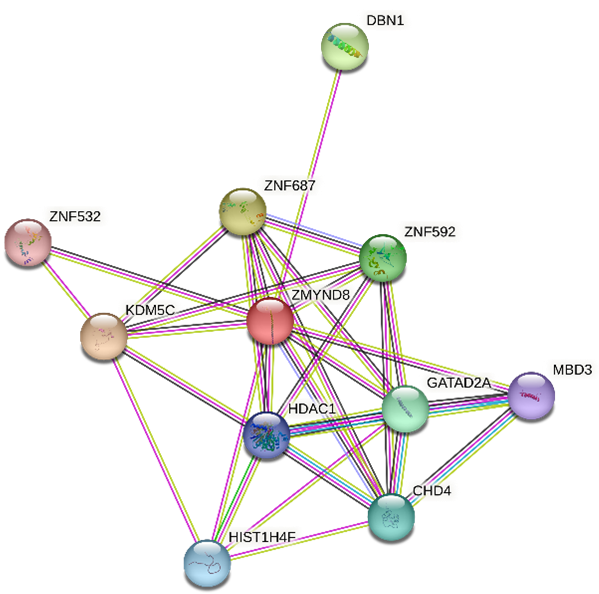
\includegraphics[width=6cm]{imagenes/interaccion.png}
	\caption{Interacciones de la proteína ZMYND8, homóloga a la proteína hipotética en cuestión. Verde: gen vecino, Rojo: Fusión de genes, Azul: gen con co-ocurrencia, Azul claro: información de bases de datos curadas, Fucsia: información determinada experimentalmente. }
	\label{18}
\end{figure}


	\begin{table}[]
		\begin{tabular}{|l|l|l|}
		\hline
		Protein  &Name  &Possible function    \\ \hline
		KDM5C& \begin{tabular}[c]{@{}l@{}}Desmetilasa 5C \\lysine specific \end{tabular} & \begin{tabular}[c]{@{}l@{}} Histona desmetilasa que\\ desmetila 	específicamente\\ 'Lys-4'\end{tabular}   \\ \hline
		ZNF687& \begin{tabular}[c]{@{}l@{}} Zinc finger \\protein 687 \end{tabular} & \begin{tabular}[c]{@{}l@{}} Puede estar involucrada\\ en regulación transcripcional   \end{tabular} \\ \hline
		DBN1& \begin{tabular}[c]{@{}l@{}} Drebrin 1  \end{tabular} & \begin{tabular}[c]{@{}l@{}} Drebrinos pueden jugar algún\\ papel en migración celular, \\extensión de procesos \\neuronales y \\plasticidad de las\\ dendritas  \end{tabular}  \\ \hline
		ZNF592& \begin{tabular}[c]{@{}l@{}} Zinc finger \\protein 592  \end{tabular} & \begin{tabular}[c]{@{}l@{}} Puede estar involucrada en\\ regulación \\ transcripcional   \end{tabular} \\ \hline
		GATAD2A& \begin{tabular}[c]{@{}l@{}} Transcriptional \\repressor \\p66-alpha  \end{tabular} & \begin{tabular}[c]{@{}l@{}}  Optimiza la represión \\mediada por MBD2  \end{tabular} \\ \hline
		CHD4& \begin{tabular}[c]{@{}l@{}} Chromodomain\\-helicase-DNA\\-binding \\protein 4  \end{tabular} & \begin{tabular}[c]{@{}l@{}} Componente del complejo\\ histona desacetilasa\\ NuRD que participa\\ en el remodelamiento \\de la cromatina \\desacetilando histonas   \end{tabular} \\ \hline
		HIST1H4F& \begin{tabular}[c]{@{}l@{}} Histone cluster\\ 1 H4 family \\member f;\\ Core component\\ of nucleosome   \end{tabular} & \begin{tabular}[c]{@{}l@{}} Las histonas juegan un rol\\ central en la regulación\\ transcripcional, \\reparación del ADN,\\ replicación del ADN y la \\ estabilidad del cromosoma.\\ Los nucleosomas envuelven\\ y compactan el ADN  en\\ cromatina.   \end{tabular} \\ \hline
		HDAC1& \begin{tabular}[c]{@{}l@{}} Histone \\deacetylase 1/2    \end{tabular} & \begin{tabular}[c]{@{}l@{}}  Responsible de desacetilar residuos\\ de lisina en la parte N-terminal\\ de las histonas centrales (H2A, \\H2B, H3 y H4). La desacetilación\\ de histonas da un tag para la \\represión epigenética y juega un\\ rol importante en la  regulación\\ transcripcional, la progresión del \\ciclo celular y el  desarrollo \\de eventos.   \end{tabular} \\ \hline
		MBD3 & \begin{tabular}[c]{@{}l@{}} Methyl-CpG\\-binding domain\\ protein 3  \end{tabular} & \begin{tabular}[c]{@{}l@{}} Actúa como un represor\\ transcripcional y \\juega un rol en el\\ silenciamiento de genes.    \end{tabular} \\ \hline
		ZNF532 & \begin{tabular}[c]{@{}l@{}} Zinc finger \\protein 532  \end{tabular} & \begin{tabular}[c]{@{}l@{}} Puede estar involucrada \\en regulación transcripcional   \end{tabular} \\ \hline
		\end{tabular}
		\end{table}

\subsection{\textbf{ Active site of the hypothetical protein}}

\begin{figure}[!h]
	\center
	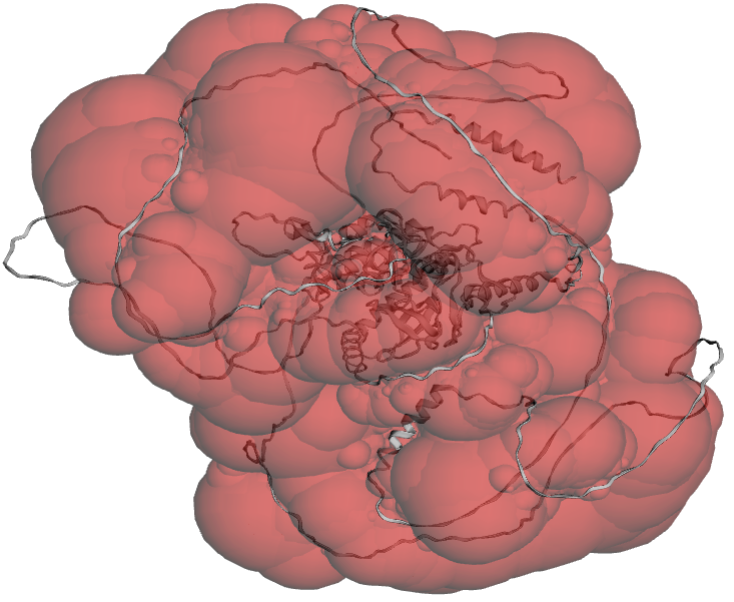
\includegraphics[width=6cm]{imagenes/activo.png}
	\caption{Interacciones de la proteína ZMYND8, homóloga a la proteína hipotética en cuestión. Verde: gen vecino, Rojo: Fusión de genes, Azul: gen con co-ocurrencia, Azul claro: información de bases de datos curadas, Fucsia: información determinada experimentalmente. }
	\label{18}
\end{figure}

   \section{Conclusion}
 
   La identificación de funciones proteicas, sobre todo en el genoma humano, es fundamental para el mejor entendimiento de procesos biológicos. Lo que puede tener impactos positivos en aplicaciones biotecnológicas y médicas. Este estudio, enfocado en identificar posibles funciones, conformaciones e interacciones, implementó múltiples herramientas bioinformáticas con las cuales se caracterizó, encontrando varias proteínas homólogas, la proteína hipotética CAI46211.1. Se encontraron funciones de unión para quinasas tipo C, actividad transductora, así como 4 motivos claramente identificados: DUF3544, Bromodominio, PHD, y PWWP. Por lo que se resalta la importancia de esta proteína hipotética en sus posibles repercusiones sobre los estudios de cáncer y se espera que se siga el análisis de esta proteína que podría influenciar los estudios de terapia de cáncer con inhibidores de bromodominios.  



\ifCLASSOPTIONcaptionsoff
  \newpage
\fi


\begin{thebibliography}{1}


 \bibitem{IEEEhowto:Monteria}
  N. Özkaya, D. Leger, D. Goldsheyder y M. Nordin, Fundamentals of Biomechanics Equilibrium, Motion, and Deformation, Switzerland: Springer, 2018. 
 

 \bibitem{IEEEhowto:Monteria}
areatecnologia., area tecnologia, [En línea]. Available: https://www.areatecnologia.com/materiales/ensayo-de-traccion.html. [Último acceso: 02 11 2022].
 \bibitem{IEEEhowto:Monteria}
E. Lawrence, INSTRON, [En línea]. Available: https://www.instron.com/en/testing-solutions/iso-standards/iso-527-2. [Último acceso: 02 11 2022].
 \bibitem{IEEEhowto:Monteria}
M. J. C. Loaiza, P. G. Díaz y e. al, Influencia de la posición de impresión y la densidad de relleno, Revista Ingenierias Universidad de Medellín, vol. 2, p. 15, 2020. 
 \bibitem{IEEEhowto:Monteria}
UMBC, UMBC, MicroMaterials Characterization Lab, [En línea]. Available: https://mmc-lab.umbc.edu/resources/instron/. [Último acceso: 02 11 2022].

 \bibitem{IEEEhowto:Monteria}
Travieso-Rodriguez JA, Jerez-Mesa R, Llumà J, Traver-Ramos O, Gomez-Gras G, Roa Rovira JJ. Mechanical Properties of 3D-Printing Polylactic Acid Parts subjected to Bending Stress and Fatigue Testing. Materials (Basel). 2019 Nov 22;12(23):3859. doi: 10.3390/ma12233859. PMID: 31766653; PMCID: PMC6926899.


\end{thebibliography}



\end{document}
